\section{Utilisation de git}

Tout au long du projet, nous avons utilisé \textit{Git} pour collaborer efficacement en groupe et organiser le travail de manière structurée.  

Chacun de nous a créé des branches dédiées au développement (\textit{dev-noe} et \textit{dev-leah}) ainsi que des branches spécifiques pour la rédaction du rapport LaTeX (\textit{rapport-noe} et \textit{rapport-leah}). Cette approche nous a permis de travailler simultanément sur différentes parties du projet, sans interférer avec les contributions des autres membres de l’équipe.  

L’utilisation des branches nous a offert une grande flexibilité : nous pouvions tester, modifier, et affiner nos contributions avant de \textit{push} et de \textit{merge} vers la branche principale (\textit{master}) une fois notre travail jugé abouti.  

Bien que nous maîtrisions déjà \textit{Git} et le travail collaboratif, ce projet nous a encore renforcé dans notre compréhension de l’importance et de l’efficacité qu’apportent les branches dans la gestion de versions et la collaboration.

\begin{center}
    \href{https://github.com/NMercierBr/PowerGridStudent/tree/master}{\textbf{Lien GitHub vers notre projet}}
    
\end{center}

\pagebreak

\vspace{1cm}

Historique des versions et visualisation des branches avec la commande \\ 
\begin{center}
    \textit{ 
        git log --graph --oneline --branches}
\end{center}

\begin{figure}[h]
    \centering
    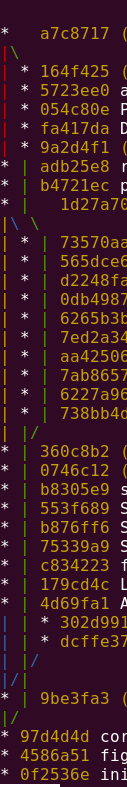
\includegraphics[width=.15\textwidth]{git/logGIT.png}
\end{figure}